\documentclass[runningheads]{llncs}

\usepackage[colorlinks=true,linkcolor = blue,urlcolor = blue]{hyperref}
\usepackage{amsmath}
\usepackage{amssymb}
\usepackage{graphicx}
\usepackage{siunitx}
\usepackage[accsupp]{axessibility}
\usepackage[table]{xcolor}

% comment out for final submission
\usepackage{ruler}
\usepackage[width=122mm,left=12mm,paperwidth=146mm,height=193mm,top=12mm,paperheight=217mm]{geometry}

\begin{document}
\pagestyle{headings}
\mainmatter
\def\ECCVSubNumber{6195}

\title{Spline-NeRF: Supplement}
\author{Anonymous ECCV Submission}
\institute{Paper ID \ECCVSubNumber}

\maketitle

\section*{Additional Qualitative Results}

We include additional qualitative results in Fig.~\ref{fig:dnerf_more} to allow for comparison of the two methods. We include these additional results in order to better visualize the qualitative differences in our method, which cannot be seen through quantitative results alone.

\section*{Voxel Spline Results}


\begin{figure}
    \vspace{-6mm}
    \centering
    \begin{minipage}[c]{0.5\textwidth}
    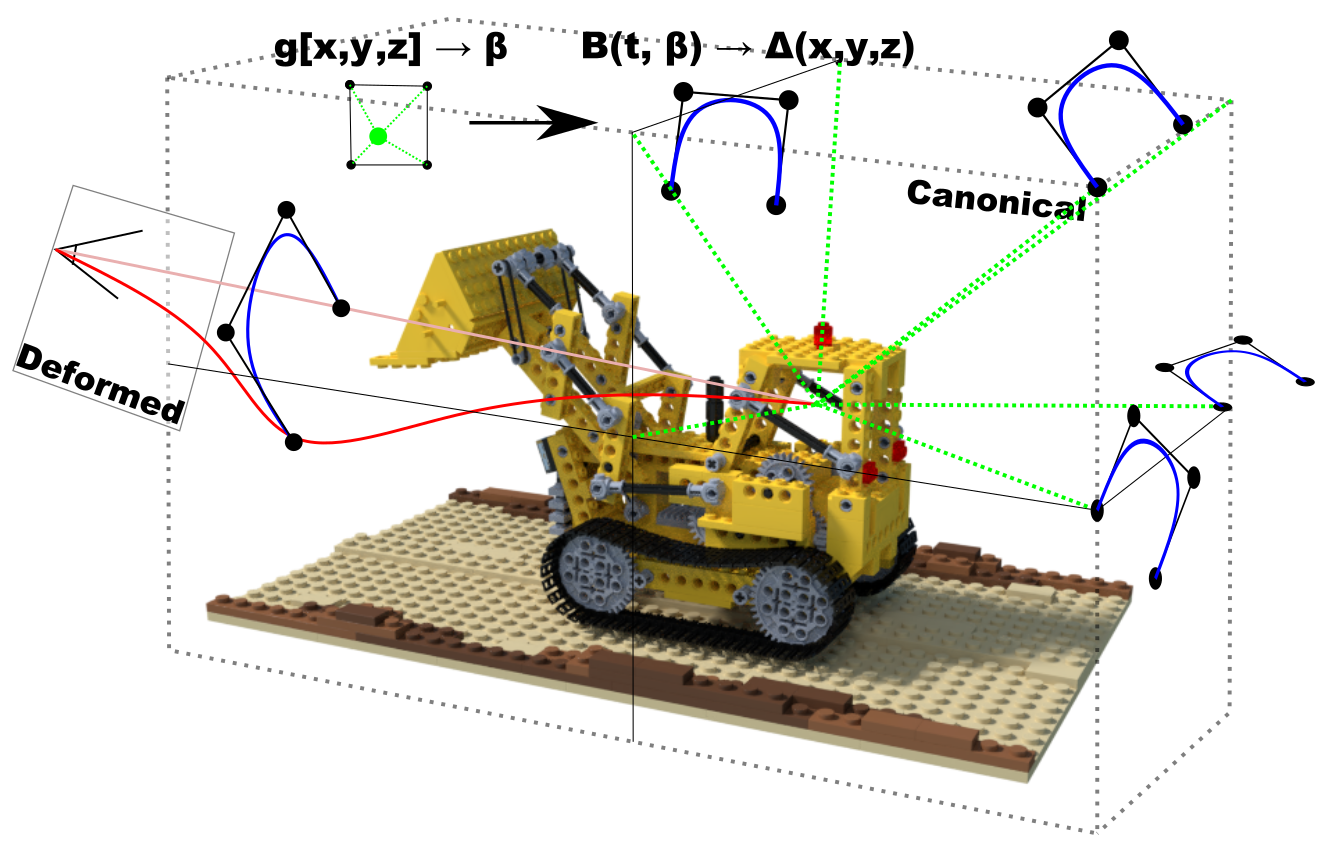
\includegraphics[width=\textwidth]{voxel_spline}
    \end{minipage}
    \begin{minipage}[c]{0.45\textwidth}
    \caption{
        \label{fig:voxel_diagram}
        \textbf{Voxel implementation of Spline-NeRF.}
        Our implementation of Spline-NeRF does not deviate much from our MLP-based implementation, but instead stores control points at each voxel coordinate.
    }
    \end{minipage}
    \vspace{-10mm}
\end{figure}

We also include some results from our naive voxel implementation in Fig.~\ref{fig:voxel_results}. We pick a few successful results to highlight that a voxel implementation can accurately recover a moving scene, but also show some failure cases to highlight that a naive voxel implementation may need additional regularization. Notably, there are a large amount of floating black spots, which is not necessarily a problem in a static reconstruction if they are not observed, but may be more of a problem if they are \textit{moved} into the line of sight. Thus, we suspect that regularization on unobserved voxels may be necessary.

Since a complete voxel implementation is not the focus of this work, we leave this for future work, but highlight its potential for fast reconstruction of dynamic scenes.




% Intended to be at the end, since it takes up a lot of space

\begin{figure*}
    \centering
    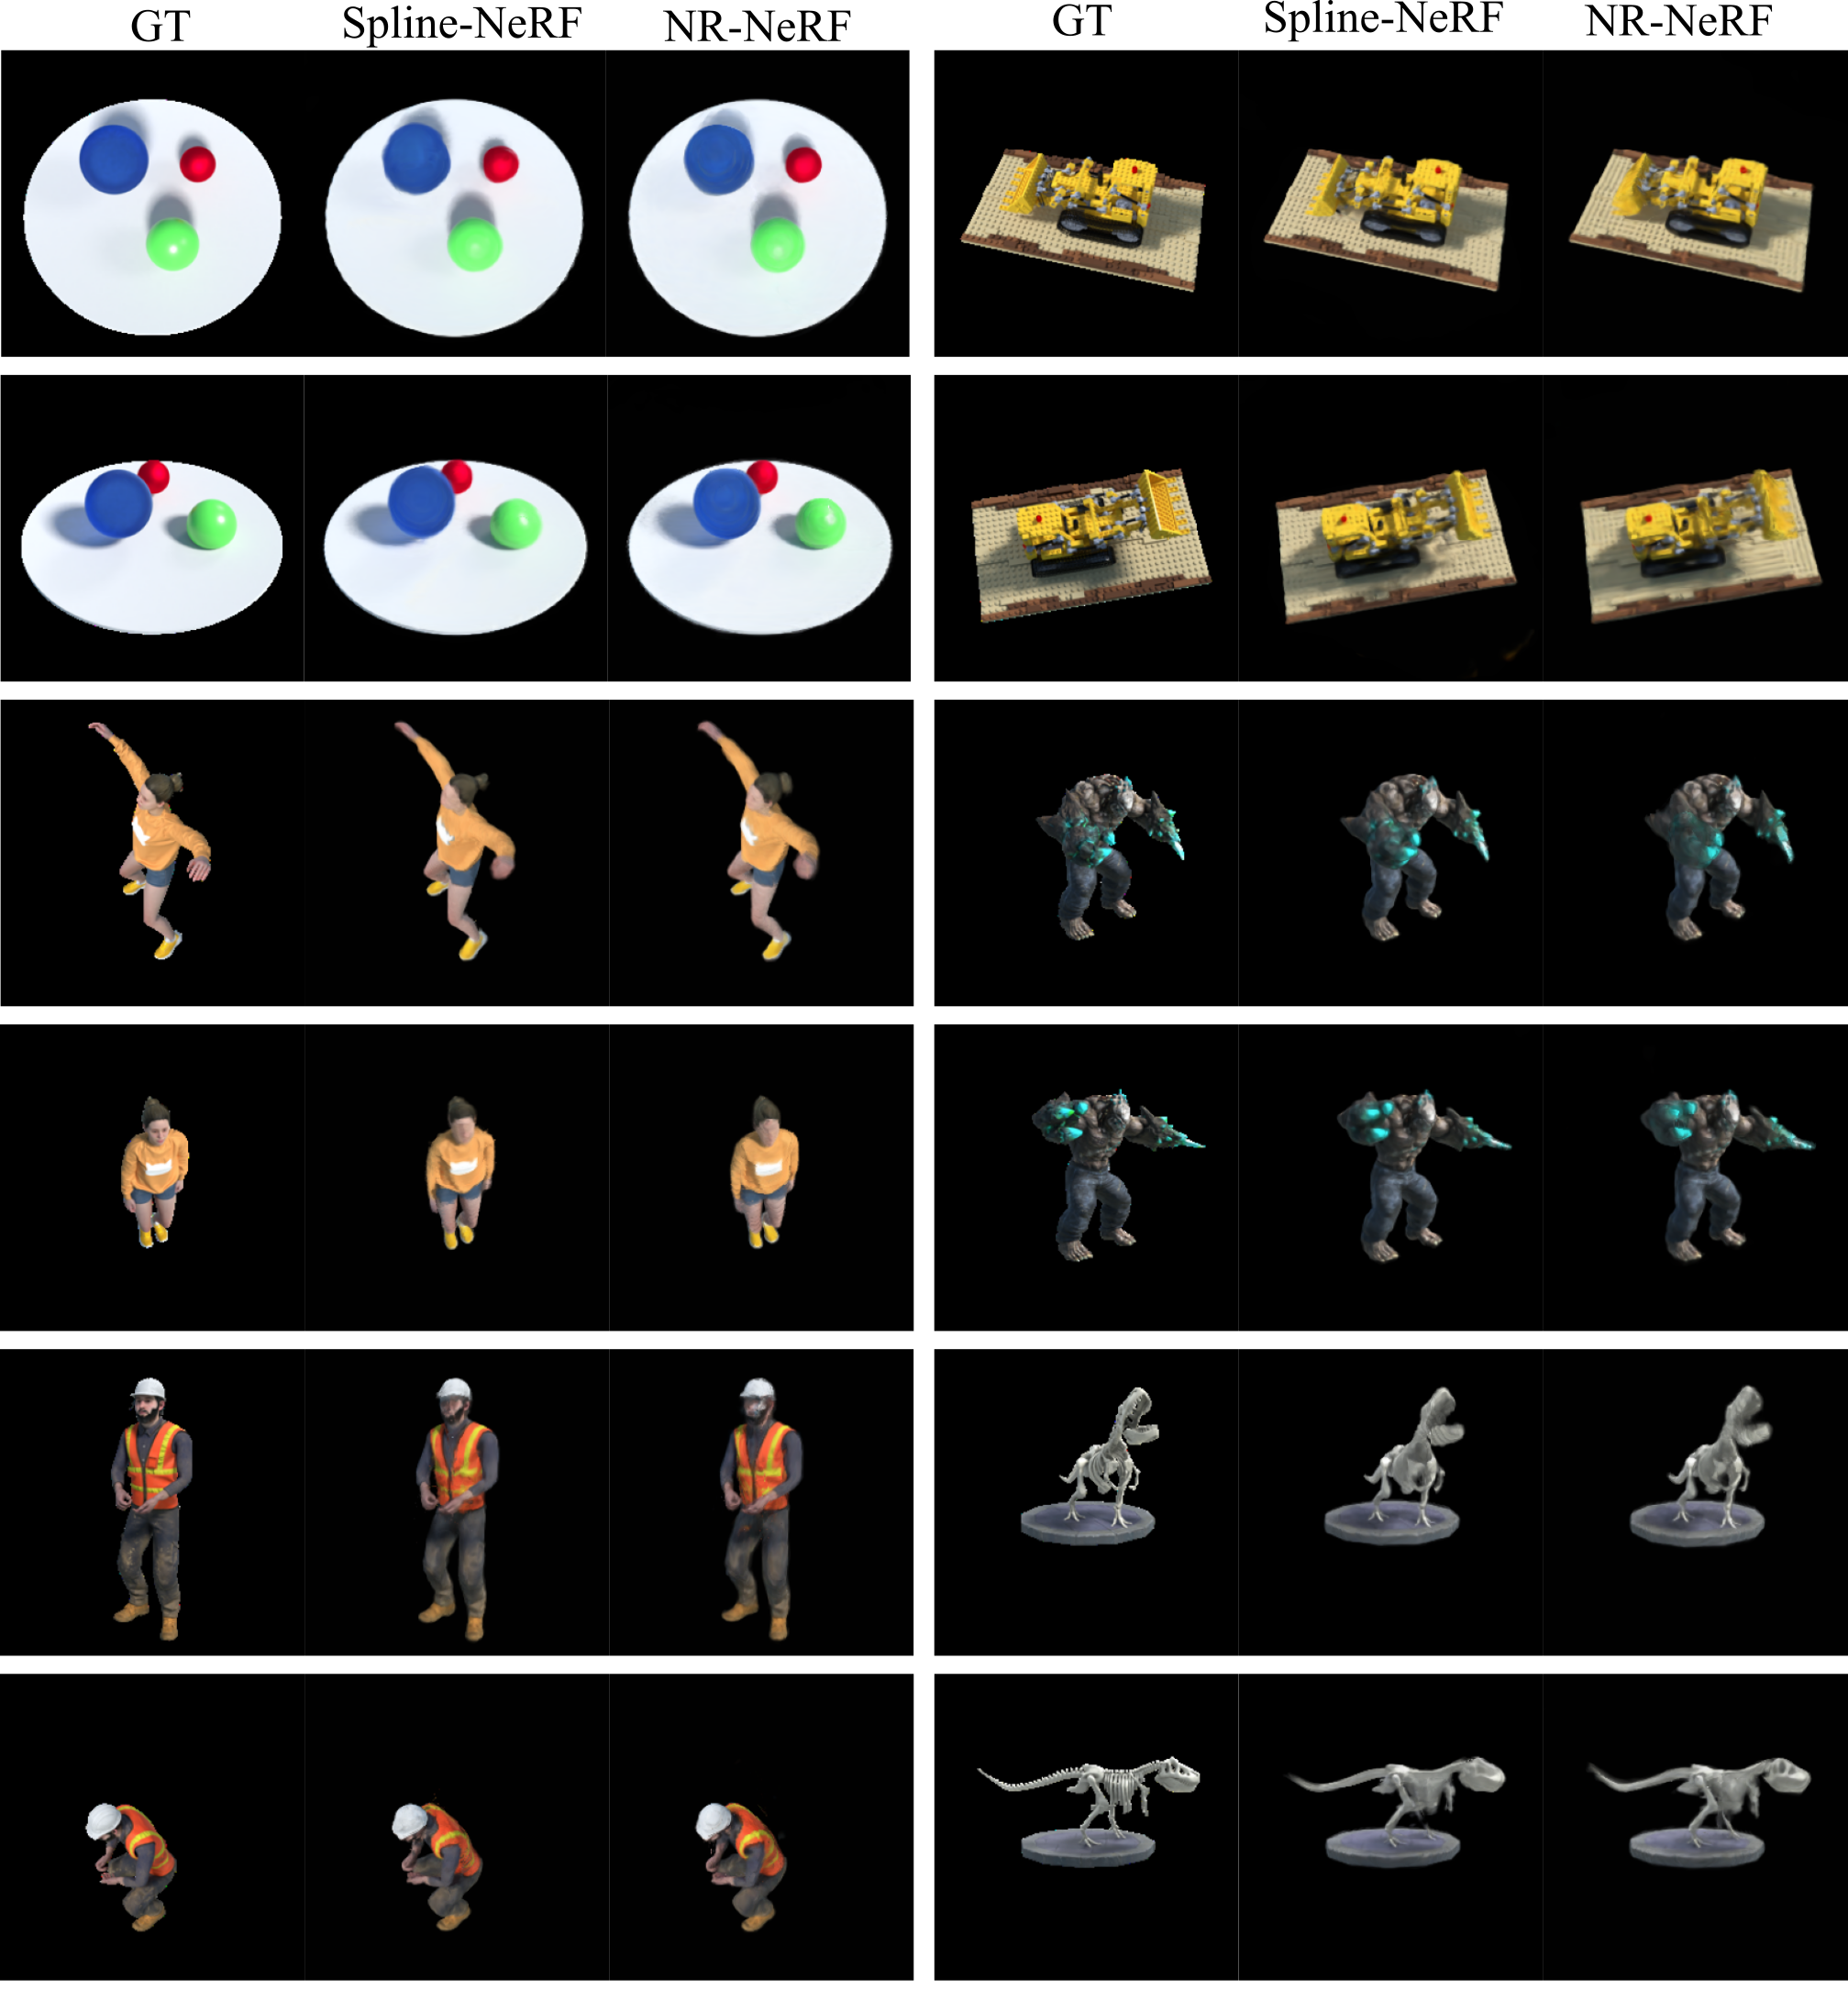
\includegraphics[width=\textwidth]{additional_results}
    \caption{
        \label{fig:dnerf_more}
        \textbf{Additional test frames from D-NeRF dataset.} More qualitative comparisons of our method to NR-NeRF. There are some cases where NR-NeRF can capture more high-quality details than Spline-NeRF, but also cases where Spline-NeRF is able to more accurately reconstruct the output. These manifest in high-frequency details, but the low-frequency components of both reconstructions are approximately the same.
    }
\end{figure*}

\begin{figure*}
    \centering
    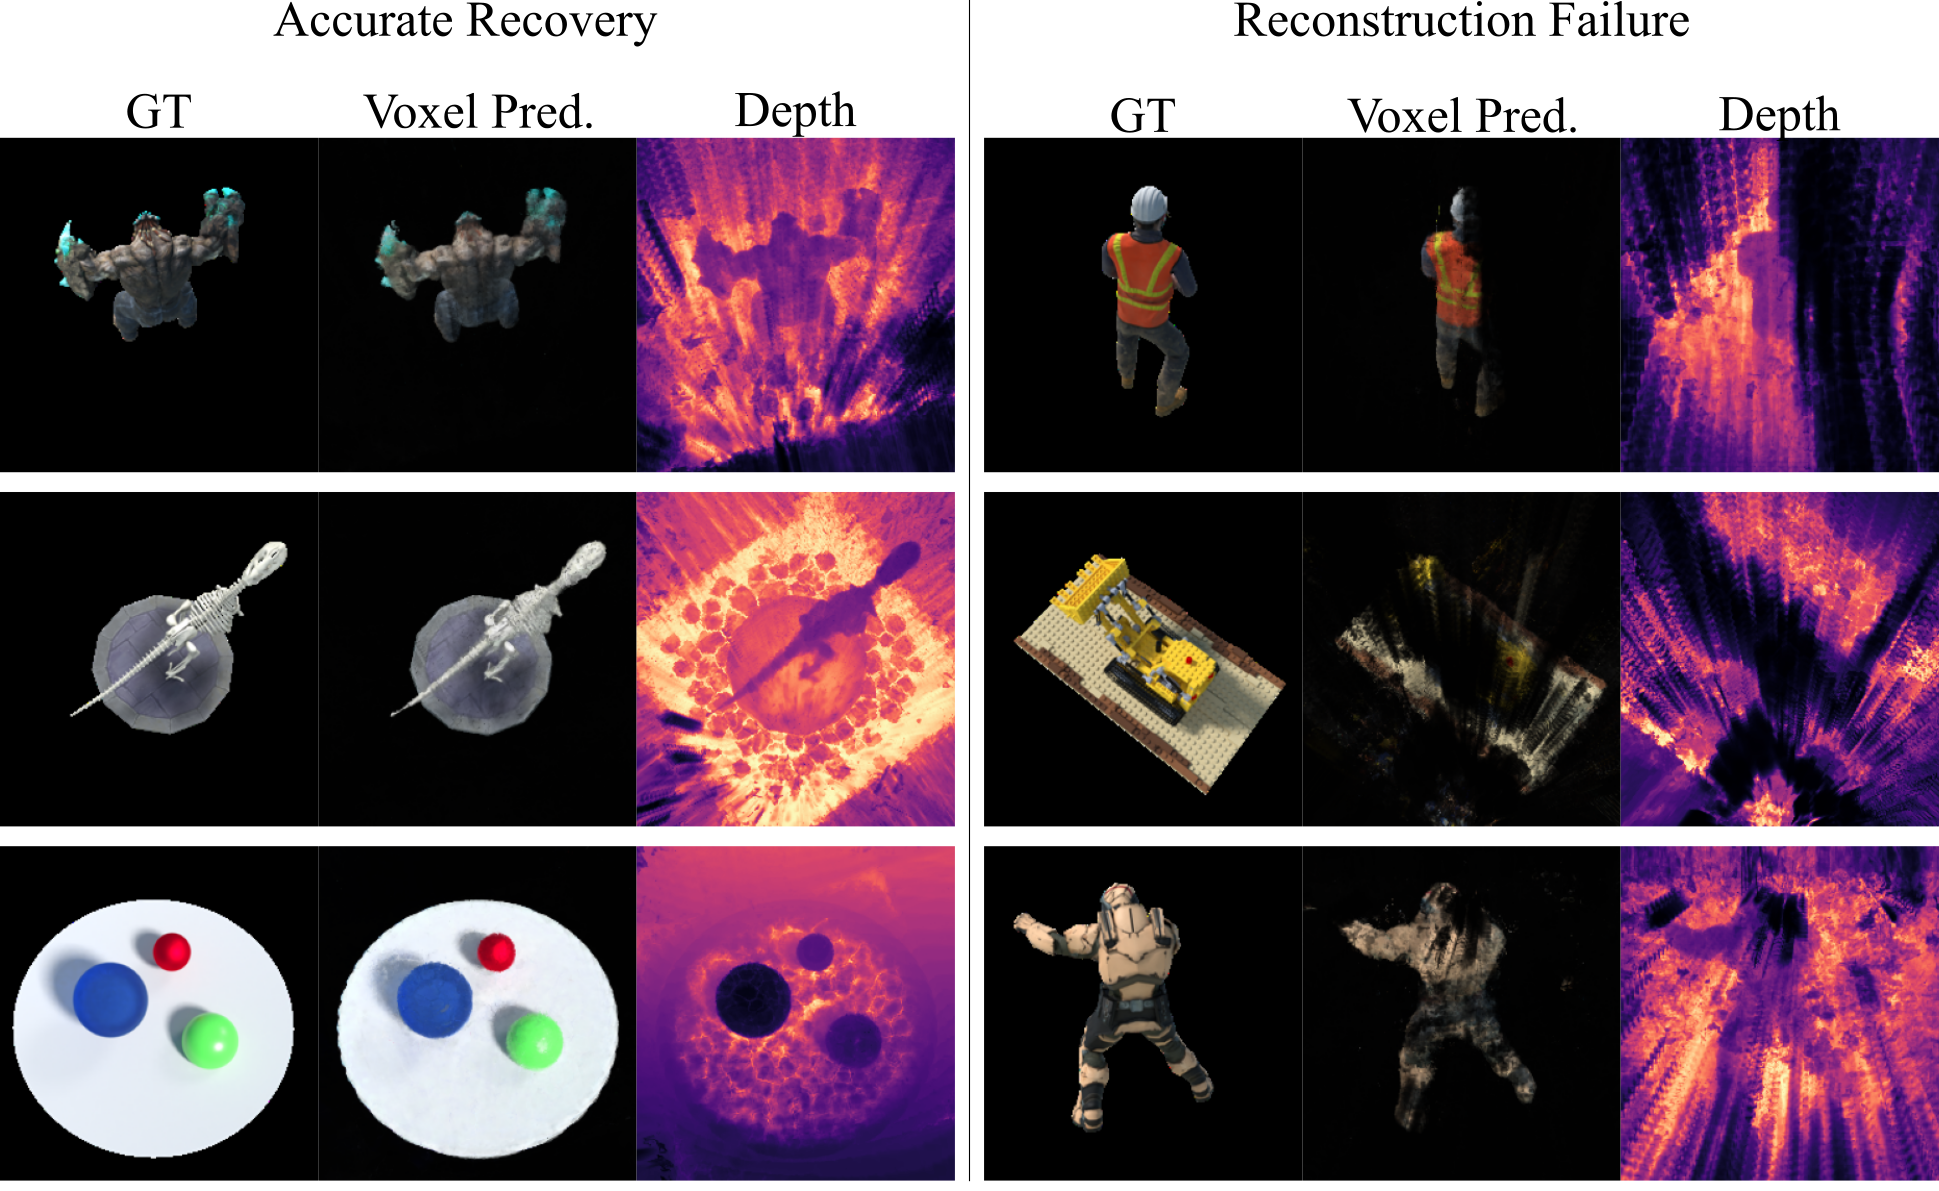
\includegraphics[width=\textwidth]{voxel_results}
    \caption{
        \label{fig:voxel_results}
        \textbf{Results from Voxel Spline-NeRF.} Results of reconstruction using a Voxel implementation of Spline-NeRF. We include both successful output from the voxel implementation, which is cherry-picked to showcase the potential of the method, as well as failure cases in order to show that there are still shortcomings without additional regularization. We note that even in the successful cases, it's clear from the visualized depth that there are artifacts, but they are black and thus do not affect the output.
    }
\end{figure*}



\end{document}